\documentclass[]{article}
\usepackage[UTF8]{ctex}
\usepackage[a4paper,left=10mm,right=10mm,bottom=10mm,top=10mm]{geometry}
\usepackage{graphicx}
\usepackage{float}
\usepackage{amsmath,amsfonts,amssymb,amsthm}
\usepackage{array,color}
%opening
\title{计算机科学中的数学基础-Exercise8}
\author{陈昱衡 521021910939}
\date{\today}

\begin{document}
\maketitle

\section*{Warmup7}
\begin{figure}[H]
    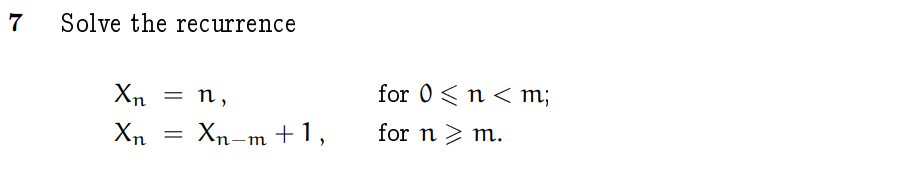
\includegraphics[scale = 0.5]{2023-03-09-10-21-58.png}
\end{figure}
由递归式的定义,可知每m个数是一一对应的,一次加一,因此可以对m个数进行整体分析,
将自然数分成连续m个数的一组,因此,n属于第$\lfloor \frac{n}{m} \rfloor$组。
\par 
n属于第几组就相对于第零组而言增加了几。\par 
于是有,
\begin{equation}
    X_{n} = \lfloor \frac{n}{m} \rfloor + n mod m
\end{equation}


\section*{Warmup8}

\begin{figure}[H]
    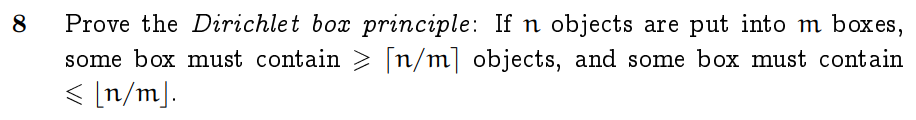
\includegraphics[scale = 0.5]{2023-03-09-10-25-13.png}
\end{figure}
此题可以运用反证法。\par 
首先考虑$\frac{n}{m}$整数的情况,此情形下显然成立。\par 
假设,每个盒子的物品数量均小于$\lceil \frac{n}{m} \rceil$,因为物品数量不能为小数,因此,
每个盒子的物品数量至多为$\lfloor \frac{n}{m} \rfloor$,故总物品数量
\begin{align}
    N \le m \times \lfloor \frac{n}{m} \rfloor
\end{align}
记$\lfloor \frac{n}{m} \rfloor$为k,则

\begin{equation}
    N \le m \times k
\end{equation}
而 $m \times k  < n$,因此推导出矛盾,定理前半部分成立。
再假设每个盒子的物品数量均大于$\lfloor \frac{n}{m} \rfloor$,借用前面证明的标记,
有每个盒子的物品数量一定至少为k+1,
则
\begin{equation}
    N \ge m \times (k+1) > n
\end{equation}
与题干中论述产生矛盾,故定理后半部分成立。\par 
定理成立。

\section*{Warmup9}
\begin{figure}[H]
    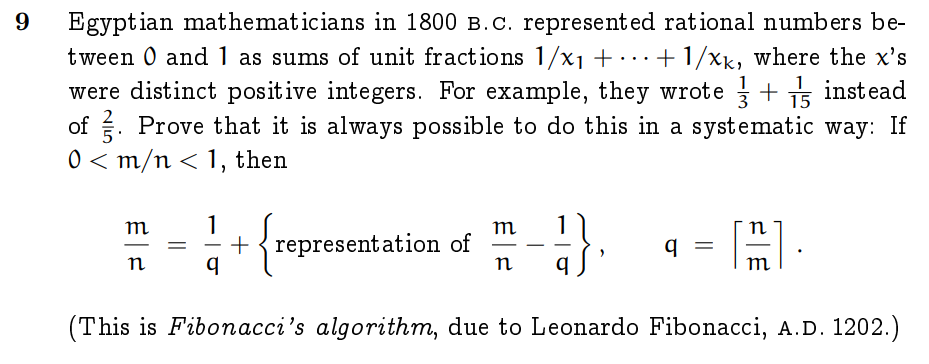
\includegraphics[scale = 0.5]{2023-03-09-10-25-44.png}
\end{figure}
借用书中的定义 $x mumble y$ = y$\lfloor \frac{x}{y} \rfloor $ - x;
可以简化斐波那契算法:
\begin{align}
    \frac{n}{m} &= \frac{1}{q} + {\frac{n}{m} - \frac{1}{q}}\\
    &= \frac{1}{q} + \frac{mq - n}{nq}
\end{align}
余项分式中的分母$mq - n$ = $n mumble m \le m$ ,而且是严格小于m。
\par 
因此,每次使用斐波那契算法转化一次,得到的数就会比上一次的分子小,且分母递增,,不相等。
\par 
故,m一定会减小到1,即得到完整的表示。

\section*{Basics10}
\begin{figure}[H]
    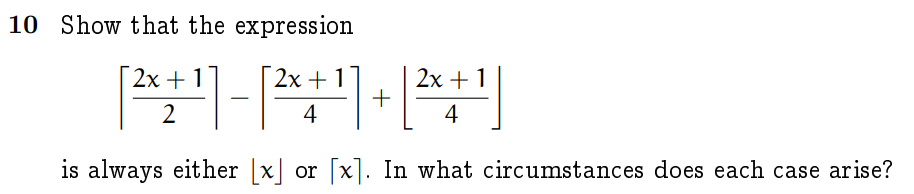
\includegraphics[scale = 0.5]{2023-03-09-10-26-04.png}
\end{figure}

我们首先将向下取整和向上取整函数中的部分取出观察。\par 
\begin{align}
    &x+\frac{1}{2} \\
    &\frac{x}{2}+\frac{1}{2} 
\end{align}
可以观察出,$\frac{x}{2}+\frac{1}{2}$的小数部分一定不会溢出进一,而$x+\frac{1}{2}$的小数分数有可能进一,以${x} = 0.5$为分界,因此,分两种情况讨论如下:
\begin{enumerate}
    \item[1] \{x\} < 0.5 \par 
    \begin{align}
        \lfloor \frac{2x+1}{2} \rfloor - \lfloor \frac{2x+1}{4} \rfloor + \lfloor \frac{2x+1}{4} \rfloor &= \lceil x \rceil - 1\\
        &= \lfloor x \rfloor
    \end{align}
    \item[2] \{x\} > 0.5 \par 
    \begin{align}
        \lfloor \frac{2x+1}{2} \rfloor - \lfloor \frac{2x+1}{4} \rfloor + \lfloor \frac{2x+1}{4} \rfloor &= \lceil x \rceil + 1 - 1\\
        &= \lceil x \rceil      
    \end{align}
    \item[3] \{x\} == 0.5 \par 
    \begin{align}
        \lfloor \frac{2x+1}{2} \rfloor - \lfloor \frac{2x+1}{4} \rfloor + \lfloor \frac{2x+1}{4} \rfloor &= \lceil x \rceil + 1 - 1\\
        &= \lceil x \rceil \\
        &= \lfloor x \rfloor     
    \end{align}

\end{enumerate}
\end{document}